% The five-stage pipelined core. Build: tectonic core.tex
\documentclass[tikz,border=3pt]{standalone}
\usepackage[T1]{fontenc}
\usepackage{mathptmx}
\usetikzlibrary{arrows.meta}
\definecolor{ipath}{HTML}{2A78D6}
\definecolor{dpath}{HTML}{EB6834}
\definecolor{ink2}{HTML}{52514E}
\definecolor{haz}{HTML}{6250D6}
\begin{document}
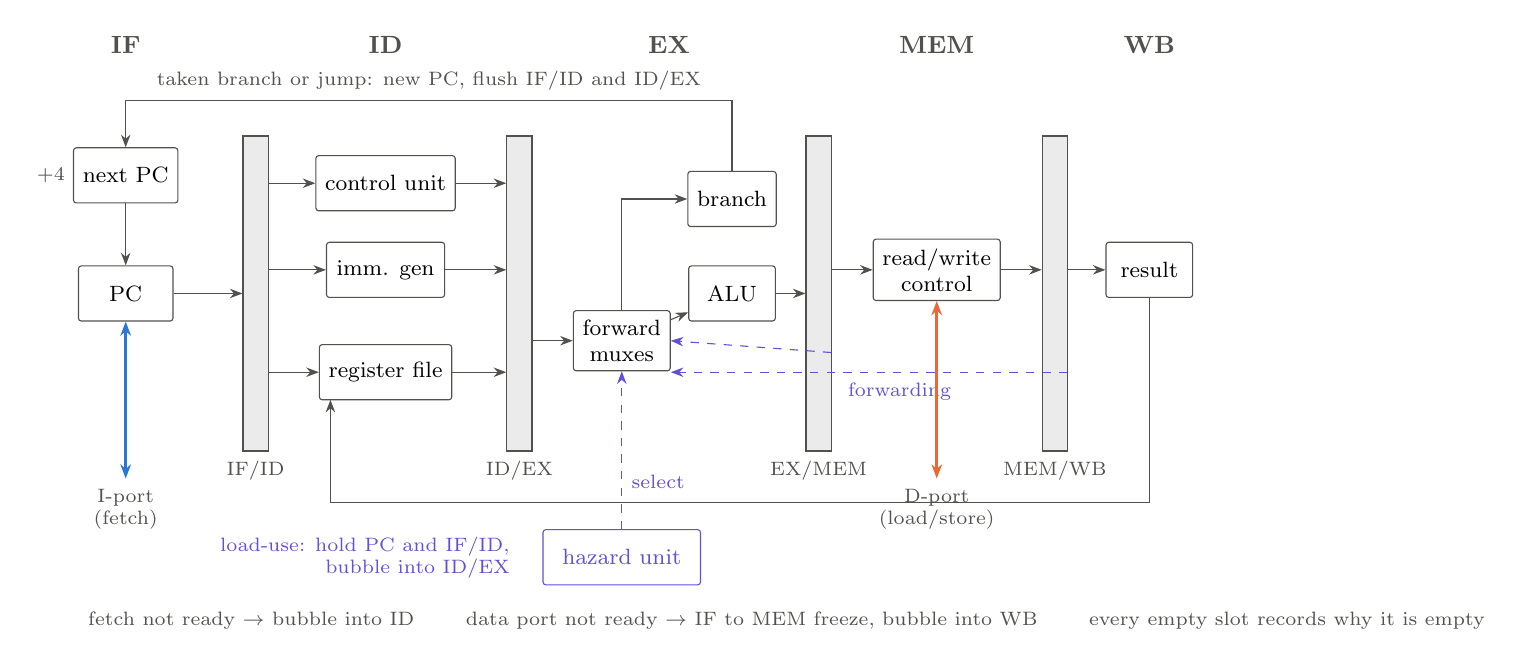
\begin{tikzpicture}[
    font=\footnotesize,
    blk/.style={draw=ink2, rounded corners=1pt, minimum width=15mm, minimum height=7mm, align=center, fill=white},
    preg/.style={draw=ink2, fill=black!8, minimum width=3.2mm, minimum height=40mm},
    arr/.style={-{Stealth[length=1.6mm]}, draw=ink2},
    fwd/.style={-{Stealth[length=1.6mm]}, draw=haz, dashed},
    ibus/.style={{Stealth[length=1.8mm]}-{Stealth[length=1.8mm]}, draw=ipath, line width=1pt},
    dbus/.style={{Stealth[length=1.8mm]}-{Stealth[length=1.8mm]}, draw=dpath, line width=1pt},
    stage/.style={font=\small\bfseries, text=ink2},
    lbl/.style={font=\scriptsize, text=ink2},
]
    % Stage names
    \node[stage] at (0.0, 4.75) {IF};
    \node[stage] at (3.3, 4.75) {ID};
    \node[stage] at (6.9, 4.75) {EX};
    \node[stage] at (10.3, 4.75) {MEM};
    \node[stage] at (13.0, 4.75) {WB};

    % Pipeline registers (bars from y = -0.4 to 3.6)
    \node[preg, label={[lbl]below:IF/ID}]  (r1) at (1.65, 1.6) {};
    \node[preg, label={[lbl]below:ID/EX}]  (r2) at (5.0, 1.6) {};
    \node[preg, label={[lbl]below:EX/MEM}] (r3) at (8.8, 1.6) {};
    \node[preg, label={[lbl]below:MEM/WB}] (r4) at (11.8, 1.6) {};

    % IF
    \node[blk, minimum width=12mm] (pcmux) at (0, 3.1) {next PC};
    \node[blk, minimum width=12mm] (pc) at (0, 1.6) {PC};
    \draw[arr] (pcmux) -- (pc);
    \draw[arr] (pc.east) -- (r1.west |- pc.east);
    \node[lbl] at (-0.95, 3.1) {$+4$};
    \draw[ibus] (pc.south) -- (0, -0.75) node[below, lbl, align=center] {I-port\\(fetch)};

    % ID
    \node[blk] (ctrl) at (3.3, 3.0) {control unit};
    \node[blk] (imm) at (3.3, 1.9) {imm. gen};
    \node[blk] (rf) at (3.3, 0.6) {register file};
    \draw[arr] (r1.east |- ctrl) -- (ctrl);
    \draw[arr] (r1.east |- imm) -- (imm);
    \draw[arr] (r1.east |- rf) -- (rf);
    \draw[arr] (ctrl) -- (r2.west |- ctrl);
    \draw[arr] (imm) -- (r2.west |- imm);
    \draw[arr] (rf) -- (r2.west |- rf);

    % EX
    \node[blk, minimum width=12mm] (fwdmux) at (6.3, 1.0) {forward\\muxes};
    \node[blk, minimum width=11mm] (alu) at (7.7, 1.6) {ALU};
    \node[blk, minimum width=11mm] (br) at (7.7, 2.8) {branch};
    \draw[arr] (r2.east |- fwdmux) -- (fwdmux);
    \draw[arr] (fwdmux) -- (alu);
    \draw[arr] (fwdmux) |- (br);
    \draw[arr] (alu) -- (r3.west |- alu);
    \draw[arr] (br.north) -- (7.7, 4.05) -- node[lbl, above] {taken branch or jump: new PC, flush IF/ID and ID/EX} (0, 4.05) -- (pcmux.north);

    % Forwarding paths into EX
    \draw[fwd] (8.96, 0.85) -- ([yshift=1.5mm]fwdmux.east |- 0, 0.85);
    \draw[fwd] (11.96, 0.6) -- (fwdmux.east |- 0, 0.6);
    \node[lbl, text=haz, anchor=west] at (9.05, 0.35) {forwarding};

    % MEM
    \node[blk, minimum width=16mm] (rw) at (10.3, 1.9) {read/write\\control};
    \draw[arr] (r3.east |- rw) -- (rw);
    \draw[arr] (rw) -- (r4.west |- rw);
    \draw[dbus] (rw.south) -- (10.3, -0.75) node[below, lbl, align=center] {D-port\\(load/store)};

    % WB
    \node[blk, minimum width=11mm] (wb) at (13.0, 1.9) {result};
    \draw[arr] (r4.east |- wb) -- (wb);
    \draw[arr] (wb.south) -- (13.0, -1.05) -- (2.6, -1.05) -- (2.6, 0.25);

    % Hazard unit
    \node[blk, draw=haz, text=haz, minimum width=20mm] (haz) at (6.3, -1.75) {hazard unit};
    \draw[fwd] (haz.north) -- node[lbl, text=haz, right, pos=0.3] {select} (fwdmux.south);
    \node[lbl, text=haz, anchor=east, align=right] at (5.0, -1.75) {load-use: hold PC and IF/ID,\\bubble into ID/EX};

    % Memory stalls
    \node[lbl, align=left, anchor=west] at (-0.6, -2.55) {fetch not ready $\rightarrow$ bubble into ID \qquad
        data port not ready $\rightarrow$ IF to MEM freeze, bubble into WB \qquad
        every empty slot records why it is empty};
\end{tikzpicture}
\end{document}
